%!TEX ROOT=../../_main.tex
Zájem o optimalizaci proudění tekutin je od nepaměti a předmětem vědeckého bádání minimálně od doby vynalezení integrálního počtu \cite{karman1997inverse}. Tato kapitola se zabývá základní definicí problému optimalizace a představuje známou, avšak v oblasti proudění tekutiny, prozatím nepříliš hojně užívanou metodu optimalizace. Dále jsou odvozeny základy této metody pro její aplikaci v druhé části této práce.
\section{Základy optimalizace}\label{sec:zaklady_opt}
Pro popis problému optimalizace se používají pojmy:
\begin{itemize}
	\item \textit{primární proměnné} $ \phi $ nebo také fyzikální veličiny či proměnné jako tlak, rychlost, teplota atd. dané většinou z konkrétních rovnic
	\item \textit{návrhové parametry} $ g $ materiálové vlastnosti, vstupní rychlost, tvar geometrie nebo hranice
	\item \textit{cílová funkce/funkcionál} $ J(\phi,g) $ hodnocení kombinace primárních a návrhových parametrů, např. tlaková ztráta, stlačení nebo vztlak
	\item \textit{vazební rovnice} $ R(\phi,g)=0 $ rovnice proudění
\end{itemize}
Problém optimalizace lze pak matematicky formulovat následovně. \cite{karman1997inverse}
\begin{problem}\label{prob:optimalizace}
Nechť je dána množina parametrů $ g=\left\lbrace g_n, \, n=1,...,N\right\rbrace $, cílová funkce $ J(\phi, g) $ a vazební rovnice $ R(\phi, g)=0 $. 
Najděte takovou kombinaci parametrů $ g $ a $ \phi $, která minimalizuje funkci $ J(\phi, g) $ a zároveň splňuje platnost podmiňujících rovnic $ R(\phi, g)=0$ . 
\end{problem}
\nomenclature[B]{$ b_n $}{Optimalizační parametry}
\nomenclature[J]{$ J $}{Cílová funkce}
\nomenclature[R]{$ R_i $}{Podmiňující rovnice}
Metod na řešení optimalizačního problému je hned několik.
Obecně je lze rozlišit na obecné a lokální optimalizační metody. Mezi všeobecně známe patři například metoda genetických algoritmu(obecná) a gradientní optimalizační metody(lokální). 
Základní rozdíl těchto metod je, že obecné optimalizační metody se zpravidla snaží přiblížit globálnímu optimu v celém prostoru přípustných parametrů, kdežto lokální metody na základě počátečního odhadu spadají do nejbližšího lokálního minima.

Typický optimalizační cyklus lokální metody lze zapsat následovně:
\begin{addmargin}[3em]{2em}% 1em left, 2em right
	\begin{description}
	\item 	Mějme počáteční odhad $ g^{(0)} $
	\item 	Pro $ n=0,1,2... $
	 	\begin{enumerate}
			\item Vyřešit $ R(\phi^{(n)},g^{(n)}) $ pro zjištění $ \phi^{(n)} $
			\item Spočítat $ \dfrac{\mathrm{d}J}{\mathrm{d}g}(\phi^{(n)},g^{(n)}) $
			\item Pomocí výsledků 1 a 2 zjistit optimální krok $ \delta g $ - např. $ \delta g = -\alpha \dfrac{\mathrm{d}J}{\mathrm{d}g}(\phi^{(n)},g^{(n)}) $
			\item Změnit návrhové proměnné $ g^{(n+1)} = g^{(n)} + \delta g $
		\end{enumerate}
	\end{description}
\end{addmargin}
Různé algoritmy se odlišují ve způsobu vyhodnocení gradientu v kroku 2. (citlivostní gradient, sdružená metoda) a následně se větví při volbě vhodného optimalizačního kroku (CGM, BFSG).  

\section{Metoda sdružené optimalizace}

Metoda sdružené optimalizace se snaží vyřešit problém popsaný v sekci \ref{sec:zaklady_opt}. 
Jde o speciální případ gradientní metody optimalizace, a tedy se předpokládá, že původní výběr optimalizovaných parametrů se nachází poměrně blízko hledaného optima. Nové, optimálnější řešení se dostane podle předpisu
\begin{equation}\label{eq:bnew_step}
g^{(n+1)}=g^{(n)}-\alpha\cdot\dfrac{\mathrm{d}J}{\mathrm{d}g}(\phi^{(n)}, \, g^{(n)}),
\end{equation}
kde $ \alpha < 0 $ je délka kroku. 
Co se týče znaménka v rovnici \ref{eq:bnew_step}, tak to je v tomto případe $ - $, neboť dle problému \ref{prob:optimalizace} hledáme minimum funkcionálu $ J $ a tedy musíme dělat krok proti směru nejvyššího růstu i.e. ve směru opačném ke gradientu.

Hlavním znakem sdružené gradientní optimalizace je způsob vyhodnocení gradientu cílové funkce vzhledem parametrům, tedy $ \frac{\mathrm{d}J}{\mathrm{d}g} $. 
Pro vyhodnocení tohoto gradientu jsou odvozeny nové parciální diferenciální rovnice (PDR).
\nomenclature[P]{PDR}{Parciální diferenciální rovnice}
Proces odvození nových PDR z metody Lagrangeových multiplikátorů, která specifikuje novou cílovou funkci, která v sobě bude zahrnovat podmiňující rovnice. 
Definujeme tak novou cílovou funkci 
\begin{equation}\label{eq:L_funkcional}
L(\phi, g,\,\xi) = J(\phi, g) + \left\langle R(\phi, g),\xi \right\rangle,
\end{equation}
kde $ \xi $ jsou tzv. sdružené proměnné (sdružené k primárním proměnným) a $  \left\langle \, \cdot\,,\cdot \,  \right\rangle $ je symetrická, bilineární forma, jejíž podoba je zpravidla jasná až z konkrétně řešeného problému.
Dostáváme tak nový problém, jehož řešení je však podle \cite{karman1997inverse} ekvivalentní s problémem \ref{prob:optimalizace}.

\begin{problem}\label{prob:Lagrange}
Nechť je dána množina parametrů $ g=\left\lbrace g_n, \, n=1,...,N\right\rbrace $, cílová funkce $ J(\phi, g) $ a vazební rovnice $ R(\phi, g)=0 $.
Najděte takovou kombinaci parametrů g, primárních proměnných $ \phi $ a sdružených proměnných $ \xi $ tak, aby $ L(\phi, g,\,\xi) = J(\phi, g) + \left\langle R(\phi, g),\xi \right\rangle$ bylo  stacionární.
\end{problem}

Z matematického hlediska je dobré podotknout, že všechny argumenty $ L $ jsou na sobě nezávislé. Pro $ J $ tomu tak nebylo, protože $ \xi $ a $ g $ spolu byli svázané přes podmiňující rovnice $ R(\phi, g)=0 $ a nešlo je tak volit nezávisle. Abychom splnili podmínku stacionarity, jak požaduje problém \ref{prob:Lagrange}, musí být variance $ L $ podle všech proměnných rovna nule.

\subsection{Optimální systém rovnic}
V této části jsou ukázány jednotlivé variace 
\begin{equation}\label{eq:L_variace}
\delta L = \delta_\xi L + \delta_\phi L + \delta_g L
\end{equation} 
pro cílovou funkci $ L $ definovanou rovnicí \ref{eq:L_funkcional}.
\subsubsection{Variace sdružených proměnných}
Nulovost variace podle sdružených proměnných $ \xi $ lze zapsat jako
\begin{equation*}
\delta_\xi L = \lim\limits_{\epsilon\rightarrow0}\dfrac{L(\phi,g,\xi+\epsilon\delta\xi)-L(\phi,g,\xi)}{\epsilon}=0,
\end{equation*}
kde variace $ \delta\xi $ je libovolná. Po dosazení za $ L $ z rovnice \ref{eq:L_funkcional}, dostáváme
\begin{equation*}
\lim\limits_{\epsilon\rightarrow0} \dfrac
{J(\phi, g) +  \left\langle\xi+\epsilon\delta\xi, R(\phi, g)\right\rangle - (J(\phi, g) +   \left\langle\xi , R(\phi, g))\right\rangle }
{\epsilon}
=0,
\end{equation*}
tedy 
\begin{equation*}
 \left\langle\delta\xi , R(\phi, g) \right\rangle = 0.
\end{equation*}
Díky libovolnosti variace $ \delta\xi $ dostáváme původní vazební rovnici 
\begin{equation}\label{eq:vazebni_rce}
R(\phi, g)=0,
\end{equation}
která tvoří první část systému optimálních rovnic. Variace podle sdružených proměnných nám z části ukázala, že stacionární bod rozšířeného funkcionálu $ L(\phi, g,\,\xi)  $ splňuje vazební rovnice.

\subsubsection{Variace primárních proměnných}
Dále vezměme variaci vzhledem ke primárním proměnným $ \phi $, tedy
\begin{equation*}
\delta_\phi L =
\lim\limits_{\epsilon\rightarrow0}
\dfrac{L(\phi+\epsilon\delta\phi,g,\xi)-L(\phi,g,\xi)}
{\epsilon}
=0
\end{equation*}
a opět po dosazení rovnice \ref{eq:L_funkcional}
\begin{equation*}
\lim\limits_{\epsilon\rightarrow0} \dfrac
{J(\phi+\epsilon\delta\phi, g) + 
 \left\langle\xi , R(\phi+\epsilon\delta\phi, g) \right\rangle -  (J(\phi, g) +  \left\langle\xi , R(\phi, g)\right\rangle)}
{\epsilon}
=0,
\end{equation*}
neboli
\begin{equation*}
\lim\limits_{\epsilon\rightarrow 0} 
\left(
\dfrac
{J(\phi+\epsilon\delta\phi, g) - J(\phi, g)}
{\epsilon}
+
\dfrac
{  \left\langle\xi , R(\phi+\epsilon\delta\phi) - R(\phi, g)\right\rangle }
{\epsilon}
\right)
=0.
\end{equation*}
Členy ve jmenovateli obsahující $ \epsilon $ přepíšeme pomocí Taylorova rozvoje okolo bodu $ \phi $
\begin{equation*}
\lim\limits_{\epsilon\rightarrow 0} 
\left(
\dfrac
{J(\phi, g) + \dfrac{\partial J}{\partial \phi}\epsilon\delta\phi + O(e^2) - J(\phi, g)}
{\epsilon}
+
\dfrac
{  \left\langle\xi , R(\phi,g) + \dfrac{\partial R}{\partial \phi} \epsilon \delta\phi + O(e^2) - R(\phi,g)\right\rangle }
{\epsilon}
\right)
=0,
\end{equation*}
kde vypadnou členy bez derivace, a po zkrácení $ \epsilon $ dostáváme
\begin{equation*}
\lim\limits_{\epsilon\rightarrow 0} 
\left(
\dfrac{\partial J}{\partial \phi}\delta\phi
+  \left\langle\xi , \dfrac{\partial R}{\partial \phi} \delta\phi \right\rangle
+O(\epsilon)
\right)
=0.
\end{equation*}
Provedeme limitu 
\begin{equation}\label{eq:sdruzene_rce_variace}
\frac{\partial J}{\partial \phi}\delta\phi
+  \left\langle\xi , \dfrac{\partial R}{\partial \phi} \delta\phi\right\rangle
=0,
\end{equation}
použijeme 
\begin{equation*}
\frac{\partial J}{\partial \phi}\delta\phi = \left\langle 1, \frac{\partial J}{\partial \phi}\delta\phi \right\rangle
\end{equation*}
a označíme $ (\cdot)^* $ sdružený operátor k $  \left\langle \, \cdot\,,\cdot \,  \right\rangle $, tedy
\begin{equation*}
\left\langle   \left(\frac{\partial J}{\partial \phi}\right)^* ,\delta\phi  \right\rangle
+  \left\langle \left(\dfrac{\partial R}{\partial \phi}\right)^* \xi ,  \delta\phi\right\rangle
=0.
\end{equation*}
Další část systému optimálních rovnic jsou tedy tzv. sdružené rovnice
\begin{equation}\label{eq:sdruzene_rce}
\left( \dfrac{\partial R}{\partial \phi} \right)^* \xi = 
- \left(\dfrac{\partial J}{\partial \phi}\right)^*.
\end{equation}

\subsubsection{Variace návrhových parametrů}

Poslední část variace $ \delta L $ je vzhledem k návrhovým parametrům $ g $, tedy
\begin{equation*}
\delta_g L =
\lim\limits_{\epsilon\rightarrow 0}
\dfrac{L(\phi,g+\epsilon\delta g,\xi)-L(\phi,g,\xi)}
{\epsilon}
=0,
\end{equation*}
kde obdobně jako pro primární proměnné po dosazení z rovnice \ref{eq:L_funkcional} dostaneme
\begin{equation*}
\lim\limits_{\epsilon\rightarrow0} \dfrac
{J(\phi, g+\epsilon\delta g) + 
	 \left\langle\xi , R(\phi, g+\epsilon\delta g)\right\rangle  -  (J(\phi, g) +  \left\langle\xi , R(\phi, g)\right\rangle)}
{\epsilon}
=0
\end{equation*}
a po aplikování stejného postupu jako pro vztah \ref{eq:sdruzene_rce}, dostaneme poslední část optimálního systému rovnic, tzv. podmínky optimálnosti
\begin{equation}\label{eq:podminky_optimalnosti}
\left( \dfrac{\partial R}{\partial g} \right)^* \xi = 
- \left(\dfrac{\partial J}{\partial g}\right)^*.
\end{equation}

\subsubsection{Řešení soustavy optimálních rovnic}
Řešením soustavy optimálních rovnic \ref{eq:vazebni_rce}, \ref{eq:sdruzene_rce} a \ref{eq:podminky_optimalnosti} dává řešení problému \ref{prob:Lagrange} a tedy i \ref{prob:optimalizace}. Analyticky lze systém vyřešit pouze ve speciálních případech a oproti základnímu systému, tedy vazebním rovnicím, je tento nesegregovaný systém často masivní, jak upozorňuje \cite{karman1997inverse}. Vyřešením této soustavy jako nesegregované dostaneme přímo optimální hodnoty návrhových parametrů, bohužel to v mnoha případech není možné. Řešení soustavy rovnic segregovaným způsobem už je schůdnější varianta, vyžaduje však iteraci a lze ukázat, že iterační metoda řešící každou z tří části odděleně je ekvivalentní k metodě nejvyššího spádu, jejíž rychlost konvergence je často nedostačující. Jak bylo již řečeno v úvodu této sekce, lze sdruženou metodu použít i jiným způsobem a to pro výpočet gradientu/variace $ \frac{\mathrm{d} J}{\mathrm{d} g} $, který je posléze použit v optimalizačním cyklu podle předpisu \ref{eq:bnew_step}.

\subsection{Gradient pomocí sdružené metody}
Získat gradient cílové funkce je v rámci optimalizačního cyklu, nastíněného na začátku této sekce, tradičně nejnáročnější operace. Gradient cílové funkce lze za použití řetízkového pravidla zapsat jako
\begin{equation}\label{eq:gradient_cilove_fce}
\dfrac
{\mathrm{d}J}
{\mathrm{d}g} (\phi^{(n)}, \, g^{(n)})
=
\dfrac
{\partial J}
{\partial \phi }(\phi^{(n)}, \, g^{(n)})
\dfrac
{\mathrm{d}\phi}
{\mathrm{d}g}(\phi^{(n)}, \, g^{(n)})
+
\dfrac
{\partial J}
{\partial g}(\phi^{(n)}, \, g^{(n)}).
\end{equation}
Mějme řešení sdružených rovnic \ref{eq:sdruzene_rce} v n-té iteraci, i.e. mějme $ \xi^{(n)} $, které řeší
\begin{equation}\label{eq:temp1}
\xi^{(n)} \cdot \dfrac{\partial R}{\partial \phi} \Bigr|_{g^{(n)}}=\dfrac{\partial J}{\partial \phi}\Bigr|_{g^{(n)}}.
\end{equation}
Dosazením \ref{eq:temp1} do rovnice \ref{eq:gradient_cilove_fce} dostaneme 
\begin{equation*}
\dfrac{\mathrm{d}J}
{\mathrm{d}g} (\phi^{(n)}, \, g^{(n)})
=
\xi^{(n)} 
\cdot 
\left(
\dfrac{\partial R}
{\partial \phi}\Bigr|_{g^{(n)}}
\right)
\dfrac{\mathrm{d}\phi}
{\mathrm{d}g}\Bigr|_{g^{(n)}}
+
\dfrac{\partial J}
{\partial g}\Bigr|_{g^{(n)}},
\end{equation*}
kam dosadíme variaci vazebních rovnic $ R(\phi,g)=0 $
\begin{equation*}
\left(
\dfrac{\partial R}
{\partial \phi}\Bigr|_{g^{(n)}}
\right)
\dfrac{\mathrm{d}\phi}
{\mathrm{d}g}\Bigr|_{g^{(n)}}
=
-\dfrac{\partial R}
{\partial g}\Bigr|_{g^{(n)}},
\end{equation*}
čímž se dopracujeme k hledanému vztahu
\begin{equation*}
\dfrac{\mathrm{d}J}
{\mathrm{d}g} (\phi^{(n)}, \, g^{(n)})
=
-\xi^{(n)} 
\cdot 
\dfrac{\partial R}
{\partial g}\Bigr|_{g^{(n)}}
+
\dfrac{\partial J}
{\partial g}\Bigr|_{g^{(n)}},
\end{equation*}
V optimalizačních úlohách se k zjištění gradientů typicky používá metoda konečných diferencí. Náročnost výpočtu ale roste přímo úměrně s počtem návrhových parametrů, kdežto ve sdružené metodě závisí vyhodnocení gradientu převážně na rychlosti výpočtu sdružených PDR. Ve sdružené metodě je pak navíc potřeba odvodit příslušné PDR a to teoreticky pro každou cílovou funkci. Prakticky lze ale určit dostatečně obecný předpis pro cílovou funkci, odvodit rovnice pro ni a konkrétní předpis dosadit až později.

\subsection{Sdružené rovnice pro proudění nestlačitelné tekutiny}

V této podsekci budou odvozeny sdružené rovnice pro tvarovou optimalizaci v nestlačitelném proudění podle \cite{papadimitriou2007continuous, furst2020mko2}. Podmiňující rovnice budou tedy NS rovnice pro stacionární stav s tekutinou o konstantní hustotě, tedy rovnice hybnosti
\begin{equation}\label{eq:rce_hybnosti}
\mathbf{R^u}=\left(\mathbf{u}\cdot\nabla\right)\mathbf{u} + \nabla p - \nabla \cdot 2 \nu D(\mathbf{u}),
\end{equation}
kde operátor $ D(\mathbf{u})=\frac{1}{2}(\nabla\mathbf{u}+\nabla\mathbf{u}^T) $, a rovnice kontinuity
\begin{equation}
R^p=-\nabla \cdot \mathbf{u}.
\end{equation}\label{eq:rce_kontinuity}
Primární proměnné jsou tedy v tomto případě rychlost $ \mathbf{u} $ a měrný tlak ve smyslu rovnice \ref{eq:NS_icoPseudotlak}, tedy $ p = \dfrac{p_{fyz}}{\rho}$. K nim budou odpovídat sdružené proměnné $ \xi = (\mathbf{v},q) $. Obecnou cílovou funkci lze v rámci mnoha inženýrských aplikací zapsat pomocí integrálu přes výpočetní oblast a integrálu přes hranici, tedy
\begin{equation}\label{eq:cenova_fce}
J(\mathbf{u},p,g)=\int_{\Omega} J_\Omega(\mathbf{u},p,g) \, \mathrm{d}V + \int_{\Gamma}J_\Gamma(\mathbf{u},p,g) \, \mathrm{d}S.
\end{equation}
S takto definovanými proměnnými, vazebními rovnicemi a cenovou funkcí lze definovat upravenou cenovou funkci
\begin{equation}
L= J + \int_\Omega \xi \cdot \mathbf{R} \,\mathrm{d}\Omega 
%= J + \int_\Omega \mathbf{v}\cdot\mathbf{R^u}+p\, R^p \,\mathrm{d}\Omega
= \int_\Omega \mathbf{v}\cdot\mathbf{R^u}+ q R^p +J_\Omega  \,\mathrm{d}\Omega + \int_{\Gamma}J_\Gamma \, \mathrm{d}S
\end{equation}
a pokračovat k odvození sdružených rovnic a definujeme vhodnou bilineární formu 
\begin{equation}
\left\langle \mathbf{a},\mathbf{b} \right\rangle = \int_{\Omega} \mathbf{a} \cdot \mathbf{b} \, \mathrm{d}V.
\end{equation} 
Vyjdeme předpisu \ref{eq:sdruzene_rce_variace} pro variaci upravené cenové funkce podle primárních proměnných
\begin{equation} \label{eq:sdruzena_variace}
\delta_\phi L = 
\frac{\partial J}{\partial \phi}\delta\phi
+
\int_{\Omega} 
\xi \cdot \dfrac{\partial R}{\partial \phi}  \delta\phi 
\, \mathrm{d}V
 = 0
\end{equation}
Pro člen s $ J $ můžeme přímo psát
\begin{align}
\dfrac{\partial J}{\partial u_i}& \delta u_i = \int_{\Omega} \dfrac{\partial J_{\Omega}}{\partial u_i} \delta u_i \, \mathrm{d}V + \int_{\Gamma} \dfrac{\partial J_{\Gamma}}{\partial u_i} \delta u_i \, \mathrm{d}S, \\
\dfrac{\partial J}{\partial p} &\delta p \,\,= \int_{\Omega} \dfrac{\partial J_{\Omega}}{\partial p} \delta p  \, \mathrm{d}V + \int_{\Gamma} \dfrac{\partial J_{\Gamma}}{\partial p} \delta p  \, \mathrm{d}S.
\end{align}
Pro člen se sdruženými proměnnými $ \xi \cdot \dfrac{\partial R}{\partial \phi} $ provedeme variaci $ \delta\phi $ postupně pro každou rovnici
\begin{gather*}
\delta_\mathbf{u} \mathbf{R^u}=
(\delta \mathbf{u}\cdot \nabla )\mathbf{u} + (\mathbf{u}\cdot \nabla )\delta\mathbf{u} - \nabla \cdot (2\nu D(\delta \mathbf{u}) ) ,\\
\delta_p \mathbf{R^u}= \nabla \delta p,\\
\delta_\mathbf{u}R^p = -\nabla \cdot \delta \mathbf{u} ,\\
\delta_p R^p = 0.
\end{gather*}
Pro úplnost je potřeba podotknout, že jsme vynechali variaci kinematické viskozity $ \nu $. 
Pro laminární proudění je to naprosto platný postup. 
Pokud ale budeme modelovat turbulenci za pomocí přídavné turbulentní vazkosti $ \nu = \nu_t + \widetilde{\nu} $, tak buďto musíme udělat předpoklad tzv. zmražené turbulence (anglicky frozen turbulence) a nebo rozepsat i variace rovnic turbulence. Zkoumání variace modelů turbulence je nad rámec této práce a detailněji se o něm píše v \cite{zymaris2009continuous}, kde se rozebírá i vliv zjednodušujícího předpokladu zmrazené turbulence na výsledek pro případ různých Reynoldsových čísel. 

Odvozené vztahy nyní dosadíme do předpisu \ref{eq:sdruzena_variace}
\begin{multline}
\delta_\phi L = 
\int_{\Omega} \dfrac{\partial J_{\Omega}}{\partial u_i} \delta u_i \, \mathrm{d}V 
+ 
\int_{\Gamma} \dfrac{\partial J_{\Gamma}}{\partial u_i} \delta u_i \, \mathrm{d}S
+
\int_{\Omega} \dfrac{\partial J_{\Omega}}{\partial p} \delta p  \, \mathrm{d}V 
+ 
\int_{\Gamma} \dfrac{\partial J_{\Gamma}}{\partial p} \delta p  \, \mathrm{d}S
+\\+
\int_{\Omega} 
		\underbrace{\mathbf{v} \cdot(\delta \mathbf{u}\cdot \nabla )\mathbf{u}}_\mathrm{I}
		+ \underbrace{\mathbf{v} \cdot(\mathbf{u}\cdot \nabla )\delta\mathbf{u}}_\mathrm{II}
		\underbrace{ - \mathbf{v} \cdot (\nabla \cdot (2\nu D(\delta \mathbf{u}) ))}_\mathrm{III}
\, \mathrm{d}V
+\\+
\underbrace{
\int_{\Omega} 
 \mathbf{v} \cdot \nabla \delta p
\, \mathrm{d}V
}_\mathrm{IV}
+
\underbrace{
\int_{\Omega} 
  - q \nabla \cdot \delta \mathbf{u}
\, \mathrm{d}V.
}_\mathrm{V} 
\end{multline}
Postupně teď pomocí Gaussovy věty (integrace per-partes) přesuneme derivace na sdružené proměnné, tak abychom mohli vytknout variace primárních proměnných. Pro odvození některých členů je výhodnější použít indexový zápis s Einstainovou sumační konvencí, tedy
\begin{equation*}
\mathrm{I}
=
\int_{\Omega} 
\mathbf{v}\cdot(\delta\mathbf{u}\cdot \nabla)\mathbf{u}
\, \mathrm{d}V
=
\int_{\Omega} 
v_j \delta u_i \frac{\partial u_j}{x_i}
\, \mathrm{d}V
\end{equation*}
a po aplikaci Gaussovy věty
\begin{equation*}
\mathrm{I}
=
\int_{\Gamma} 
v_j \delta u_i u_j n_i
\, \mathrm{d}S
-
\int_{\Omega} 
\frac{\partial( v_j \delta u_i )}{x_i}u_j
\, \mathrm{d}V,
\end{equation*}
rozepíšeme derivaci součinu
\begin{equation*}
\mathrm{I}
=
\int_{\Gamma} 
v_j \delta u_i u_j n_i
\, \mathrm{d}S
-
\int_{\Omega} 
v_j\underbrace{\frac{\partial( \delta u_i )}{x_i}u_j}_{=0 \text{ z kontinuity} }
\, \mathrm{d}V,
-
\int_{\Omega} 
\delta u_i \frac{\partial v_j  }{x_i}u_j
\, \mathrm{d}V
\end{equation*} 
a tedy
\begin{equation}\label{eq:clen_I}
\mathrm{I}
=
\int_{\Gamma} 
v_j u_j n_i \delta u_i 
\, \mathrm{d}S
-
\int_{\Omega} 
\frac{\partial v_j  }{x_i} u_j \delta u_i
\, \mathrm{d}V
=
\int_{\Gamma} 
(\mathbf{v}\cdot \mathbf{u} )\mathbf{n} \cdot \delta\mathbf{u}
\, \mathrm{d}S
-
\int_{\Omega} 
(\nabla \mathbf{v}\cdot \mathbf{u})\cdot\delta \mathbf{u}
\, \mathrm{d}V.
\end{equation}
Pro druhý člen můžeme psát
\begin{equation*}
\mathrm{II}
=
\int_{\Omega} 
\mathbf{v}\cdot(\mathbf{u}\cdot \nabla)\delta\mathbf{u}
\, \mathrm{d}V
=
\int_{\Omega} 
v_j  u_i \frac{\partial (\delta u_j)}{x_i}
\, \mathrm{d}V
\end{equation*}
a stejným postupem jako v předchozím případě (Gaussova věta, derivace součinu, rovnice kontinuity) dostáváme
\begin{equation}\label{eq:clen_II}
\mathrm{II}
=
\int_{\Gamma} 
v_j u_i n_i \delta u_j  
\, \mathrm{d}S
-
\int_{\Omega} 
u_i \frac{\partial v_j  }{x_i} \delta u_j
\, \mathrm{d}V
=
\int_{\Gamma} 
(\mathbf{n} \cdot \mathbf{u}) \mathbf{v}\cdot \delta \mathbf{u} 
\, \mathrm{d}S
-
\int_{\Omega} 
(\mathbf{u} \cdot \nabla)\mathbf{v}\cdot \delta \mathbf{u}
\, \mathrm{d}V.
\end{equation}
Nejpracnější je pak člen číslo tři, tedy
\begin{equation*}
\mathrm{III}
=
\int_{\Omega} 
-\mathbf{v}\cdot \left(\nabla \cdot (2\nu D(\delta \mathbf{u}) )\right)
\, \mathrm{d}V
=
\int_{\Omega} 
- v_i \frac{\partial}{\partial x_j} \left(  \nu
\left(\frac{\partial (\delta \mathbf{u}_i)}{\partial x_j} + 
\frac{\partial (\delta \mathbf{u}_j)}{\partial x_i}\right)
\right)
\, \mathrm{d}V,
\end{equation*}
použijeme Gaussovu větu poprvé
\begin{equation*}
\mathrm{III}
=
\int_{\Gamma} 
- v_i \left(  \nu
\left(\frac{\partial (\delta \mathbf{u}_i)}{\partial x_j} + 
\frac{\partial (\delta \mathbf{u}_j)}{\partial x_i}\right)
\right) n_j
\, \mathrm{d}S
+
\int_{\Omega} 
\frac{\partial v_i}{\partial x_j}   \nu
\left(\frac{\partial (\delta \mathbf{u}_i)}{\partial x_j} + 
\frac{\partial (\delta \mathbf{u}_j)}{\partial x_i}\right)
\, \mathrm{d}V
\end{equation*}
a podruhé, zvlášť na oba členy v objemovém integrálu,
\begin{multline*}
\mathrm{III}
=
\int_{\Gamma} 
- 2\nu \mathbf{v} \cdot  D(\delta \mathbf{u})\cdot \mathbf{n}
\, \mathrm{d}S
+
\int_{\Gamma} 
\nu \frac{\partial v_i}{\partial x_j}
(n_j \delta u_i + n_i \delta u_j)
\, \mathrm{d}S
-\\-
\int_{\Omega} 
\frac{\partial}{\partial x_j}\left( \nu \frac{\partial v_i}{\partial x_j} \right) \delta u_i + \frac{\partial}{\partial x_i}\left( \nu \frac{\partial v_i}{\partial x_j} \right) \delta u_j
\, \mathrm{d}V,
\end{multline*}
čímž dostáváme výraz
\begin{equation}\label{eq:clen_III}
\mathrm{III}
=
\int_{\Gamma} 
2\nu \mathbf{n} \cdot  D(\mathbf{v})\cdot \delta \mathbf{u}
\, \mathrm{d}S
- \int_{\Gamma} 
2\nu \mathbf{v} \cdot  D(\delta \mathbf{u})\cdot \mathbf{n}
\, \mathrm{d}S
-
\int_{\Omega} 
\nabla \cdot \left( 2\nu D(\mathbf{v}) \right) \cdot \delta \mathbf{u}
\, \mathrm{d}V.
\end{equation}
Dále
\begin{equation*}
\mathrm{IV}
=
\int_{\Omega} 
\mathbf{v} \cdot \nabla \delta p
\, \mathrm{d}V
=
\int_{\Omega} 
v_i \frac{\partial (\delta p) }{\partial x_i}
\, \mathrm{d}V
=
\int_{\Gamma} 
v_i n_i \delta p 
\, \mathrm{d}S
-
\int_{\Omega} 
 \frac{\partial v_i }{\partial x_i} \delta p
\, \mathrm{d}V
\end{equation*}
a 
\begin{equation}\label{eq:clen_IV}
\mathrm{IV}
=
\int_{\Gamma} 
\mathbf{v}\cdot \mathbf{n} \delta p 
\, \mathrm{d}S
-
\int_{\Omega} 
\nabla \cdot \mathbf{v} \delta p
\, \mathrm{d}V.
\end{equation}
Pro poslední člen pak
\begin{equation*}
\mathrm{V}
=
\int_{\Omega} 
- q \nabla \cdot \delta \mathbf{u}
\, \mathrm{d}V
=
\int_{\Omega} 
- q \frac{\partial (\delta u_i)}{\partial x_i}
\, \mathrm{d}V
= 
\int_{\Gamma} 
- q \delta u_i n_i
\, \mathrm{d}S
+
\int_{\Omega} 
 \frac{\partial q}{\partial x_i} \delta u_i
\, \mathrm{d}V
\end{equation*}
a vektorově tedy
\begin{equation}\label{eq:clen_V}
\mathrm{V}
=
\int_{\Gamma} 
- q \delta \mathbf{u \cdot n}
\, \mathrm{d}S
+
\int_{\Omega} 
\nabla q \cdot \delta \mathbf{u}
\, \mathrm{d}V.
\end{equation}

Konečně lze tedy rozepsat rovnici \ref{eq:sdruzena_variace} pomocí odvozených členů
\begin{multline*}
\delta_\phi L = 
\int_{\Omega} \dfrac{\partial J_{\Omega}}{\partial u_i} \delta u_i \, \mathrm{d}V 
+ 
\int_{\Gamma} \dfrac{\partial J_{\Gamma}}{\partial u_i} \delta u_i \, \mathrm{d}S
+
\int_{\Omega} \dfrac{\partial J_{\Omega}}{\partial p} \delta p  \, \mathrm{d}V 
+ 
\int_{\Gamma} \dfrac{\partial J_{\Gamma}}{\partial p} \delta p  \, \mathrm{d}S
+\\+
\int_{\Gamma} 
(\mathbf{v}\cdot \mathbf{u} )\mathbf{n} \cdot \delta\mathbf{u}
\, \mathrm{d}S
-
\int_{\Omega} 
(\nabla \mathbf{v}\cdot \mathbf{u})\cdot\delta \mathbf{u}
\, \mathrm{d}V
+
\int_{\Gamma} 
(\mathbf{n} \cdot \mathbf{u}) \mathbf{v}\cdot \delta \mathbf{u} 
\, \mathrm{d}S
-
\int_{\Omega} 
(\mathbf{u} \cdot \nabla)\mathbf{v}\cdot \delta \mathbf{u}
\, \mathrm{d}V
+\\+
\int_{\Gamma} 
2\nu \mathbf{n} \cdot  D(\mathbf{v})\cdot \delta \mathbf{u}
\, \mathrm{d}S
- \int_{\Gamma} 
2\nu \mathbf{v} \cdot  D(\delta \mathbf{u})\cdot \mathbf{n}
\, \mathrm{d}S
-
\int_{\Omega} 
\nabla \cdot \left( 2\nu D(\mathbf{v}) \right) \cdot \delta \mathbf{u}
\, \mathrm{d}V
+\\+
\int_{\Gamma} 
\mathbf{v}\cdot \mathbf{n} \delta p 
\, \mathrm{d}S
-
\int_{\Omega} 
\nabla \cdot \mathbf{v} \delta p
\, \mathrm{d}V
+
\int_{\Gamma} 
- q \delta \mathbf{u \cdot n}
\, \mathrm{d}S
+
\int_{\Omega} 
\nabla q \cdot \delta \mathbf{u}
\, \mathrm{d}V
\end{multline*}
a poté co dáme k sobě členy se stejnou variací a typem integrálu
\begin{align*}
\delta_\phi L = 
&\int_{\Omega} 
\left(
\dfrac{\partial J_{\Omega}}{\partial \mathbf{u}}
- \nabla \mathbf{v}\cdot \mathbf{u}
- (\mathbf{u} \cdot \nabla)\mathbf{v}
- \nabla \cdot \left( 2\nu D(\mathbf{v}) \right)
+ \nabla q
\right)
\cdot \delta \mathbf{u}
\, \mathrm{d}V
\\+
&\int_{\Gamma}
\left(
\dfrac{\partial J_{\Gamma}}{\partial \mathbf{u}}
+ (\mathbf{v}\cdot \mathbf{u} )\mathbf{n} 
+ (\mathbf{n} \cdot \mathbf{u}) \mathbf{v}
+ 2\nu \mathbf{n} \cdot  D(\mathbf{v})
- q \mathbf{n}
\right)
\cdot \delta \mathbf{u}
\, \mathrm{d}S
\\-
&\int_{\Gamma} 
2\nu \mathbf{v} \cdot  D(\delta \mathbf{u})\cdot \mathbf{n}
\, \mathrm{d}S,
\\+
&\int_{\Omega} 
\left(
\frac{\partial J_\Omega}{\partial p}
- \nabla \cdot \mathbf{v}
\right)
\delta p
\, \mathrm{d}V
\\+
&\int_{\Gamma}
\left(
\frac{\partial J_\Gamma}{\partial p}
+ \mathbf{v} \cdot \mathbf{n}
\right)
 \delta p
\, \mathrm{d}S
\end{align*}
dostáváme stejný výraz jako je odvozen v \cite{othmer2008continuous}.

Podmínka $ \delta_\phi L $ musí být splněna pro libovolnou variaci primárních proměnných. Z objemových integrálů nám tedy vychází sdružené NS rovnice pro nestlačitelnou tekutinu ve stacionárním stavu, které můžeme zapsat jako
\begin{align}
2D(\mathbf{v})\mathbf{u}
+ \nabla \cdot \left( 2\nu D(\mathbf{v}) \right)
- \nabla q 
=
\dfrac{\partial J_{\Omega}}{\partial \mathbf{u}} 
\\
\nabla \cdot \mathbf{v} 
= 
\frac{\partial J_\Omega}{\partial p},
\end{align}
kde jsme použili  
\begin{equation*}
\nabla \mathbf{v}\cdot \mathbf{u}
+ (\mathbf{u} \cdot \nabla)\mathbf{v} 
=
\frac{\partial v_j}{\partial x_i}  u_j + u_j  \frac{\partial v_i}{\partial x_j} 
=
2\cdot\frac{1}{2}
\left(
\frac{\partial v_j}{\partial x_i}
+ \frac{\partial v_i}{\partial x_j} 
\right)
u_j
=
2D(\mathbf{v})\mathbf{u}.
\end{equation*}
Hraniční integrály nám pak dávají návod na sestavení okrajových podmínek pro sdružené rovnice a to tak, aby
\begin{align}
\label{eq:sdruzenaOP1}
\int_{\Gamma}
\left(
\dfrac{\partial J_{\Gamma}}{\partial \mathbf{u}}
+ (\mathbf{v}\cdot \mathbf{u} )\mathbf{n} 
+ (\mathbf{n} \cdot \mathbf{u}) \mathbf{v}
+ 2\nu \mathbf{n} \cdot  D(\mathbf{v})
- q \mathbf{n}
\right)
\cdot \delta \mathbf{u}
\, \mathrm{d}S
&= 
\int_{\Gamma} 
2\nu \mathbf{v} \cdot  D(\delta \mathbf{u})\cdot \mathbf{n}
\, \mathrm{d}S
\\
\label{eq:sdruzenaOP2}
\int_{\Gamma}
\left(
\frac{\partial J_\Gamma}{\partial p}
+ \mathbf{v} \cdot \mathbf{n}
\right)
\delta p
\, \mathrm{d}S
&= 0.
\end{align}
Systém sdružených rovnic nápadně připomíná původní systém NS rovnic pro nestlačitelné tekutiny. Mezi zásadní rozdíly patří linearita rovnic a také, že v porovnání s původními NS rovnicemi má konvektivní člen opačné znaménko. To značí, že informace se v šíří proti směru primární rychlosti $ \mathbf{u} $ namísto po směru proudu. Sdružené rovnice často bývají o něco jednodušší, neboť existuje celá řada cenových funkcí, které závisí pouze na hraničních hodnotách. Ku příkladu třecí ztráty, výslednice sil na těleso nebo stlačení. Pro takové cílové funkce pak odpadávají pravé strany sdružených rovnic, neboť $ J_\Omega = 0 $.


\section{Pohyb sítě}

Nastinit nekolik moznych zpusobu, popsat vic zpusob pomoci obecneho prevodu na B-spliny z OF

Prozatím jsme pracovali s obecnými návrhovými parametry $ g $. V rámci zaměření a cíle této práce je nyní konkretizujeme. Pro tvarovou optimalizaci má smysl definovat návrhové parametry, které jsou svázané s tvarem výpočetní oblasti. Například pro křídlo letadla budeme chtít měnit profil, pro optimalizaci ztrát v koleni potrubí pak tvar samotného kolene atp. Pro tuto práci budeme později uvažovat kompresorovou mříž a měnit se tedy bude tvar lopatky.

První přístup co přichází v úvahu je brát přímo souřadnice bodů profilu jako návrhové parametry. To ovšem znamená spoustu návrhových parametrů, jejíchž počet při zjemňování sítě roste. V případě metody sdružené optimalizace to vlastně nevadí. Právě naopak bychom těžili tu největší výhodu sdružené optimalizace, tedy (téměř) nezávislost rychlosti výpočtu gradientu optimalizace na počtu návrhových proměnných. Druhým, už horším avšak stále řešitelným problémem, je zachování platnosti a funkčnosti výpočetní sítě. Snadno se dá představit, že při pohybu pouze hranice, se mohou začít stěny křížit, vznikat záporné objemy apod. Takovou situaci lze řešit dodatečným výpočtem a posunem i ostatních ovlivněných bodů. 

Lepším a obecně lépe fungujícím způsobem je podle \cite{adjoint2020foam} využít parametrizace oblasti pomocí objemových B-spline.
Po vydefinování sítě řídících bodů jak ukazuje například obrázek \ref{fig:zrcatko}, je každý z bodů sítě namapován z kartézského prostoru $ \mathcal{R}^3(x,y,z) $ do parametrického prostoru $ \mathcal{R}^3(u,v,w) $.
Objemové B-spline pak definují zobrazení z parametrického prostoru do kartézského. 
Matematický popis tohoto postupu je detailněji popsán v \cite{papoutsis2015noise}. 

V rámci optimalizace jsou jako návrhové parametry brány souřadnice řídících bodů objemových B-spline. Na základě získaných gradientů se nejprve pohne s řídícími body a následně se změna propaguje na každý parametrizovaný bod v kartézském prostoru sítě.

\begin{figure}
	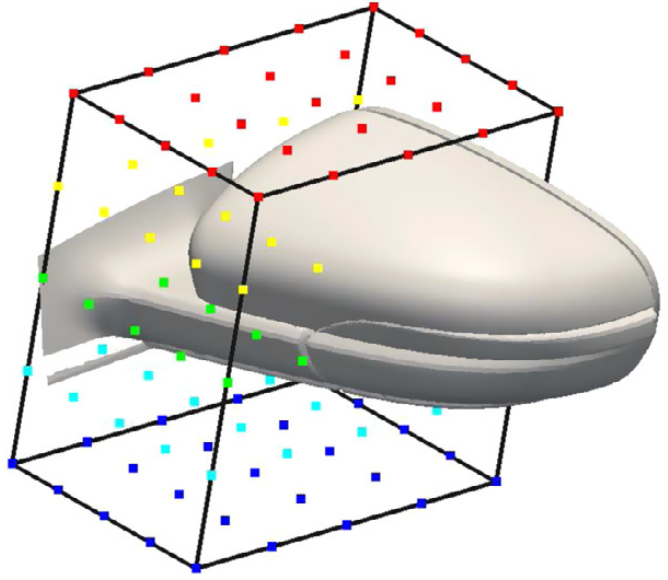
\includegraphics[width=0.7\textwidth]{./img/ridici_body.png}
	\caption{Řídící body objemového B-spline okolo automobilového zrcátka. Příklad z \cite{papoutsis2015noise}.}
	\label{fig:zrcatko}
\end{figure}


\section{Optimalizacni cyklus}

flowchart s naznacenim kde kdy se jake rovnice pocitaji (hlavni NS-rce, sdruzene rce, pohyb site)

\begin{figure}
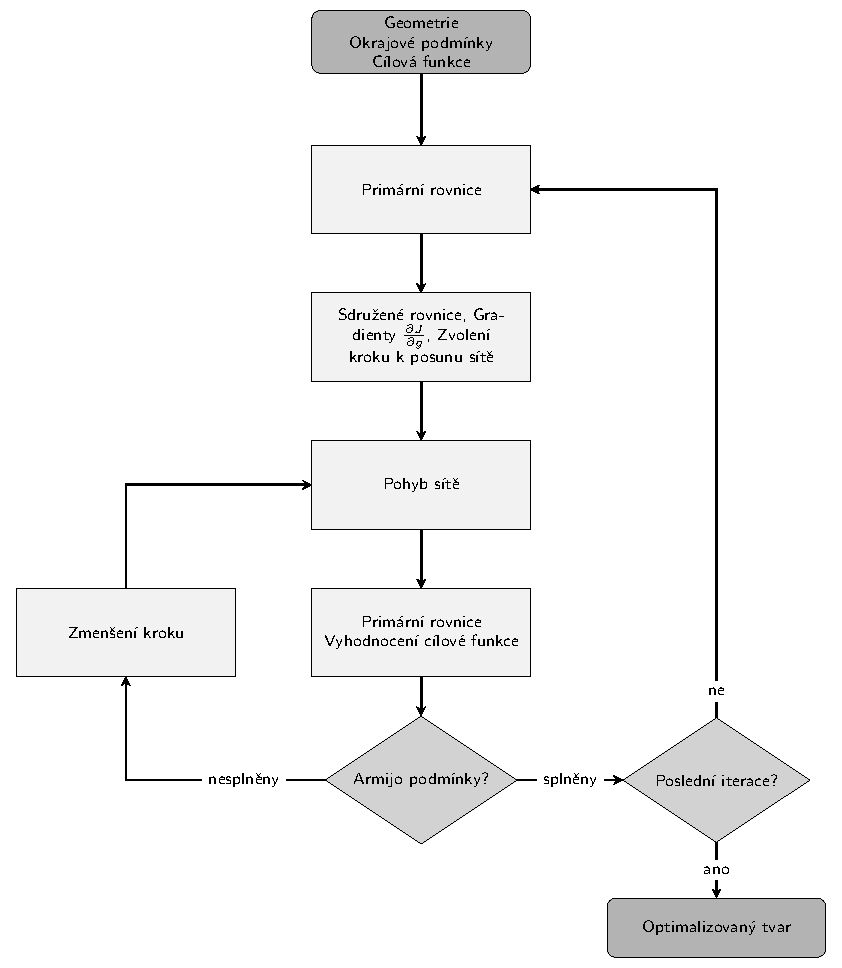
\includegraphics[width=0.9\textwidth]{./img/flowchart/optimalizacni_cyklus.pdf}
\caption{Optimalizacni cyklus}
\label{fig:flowchart_opt_cyklus}
\end{figure}

